\chapter{Purely quantum light}\label{chap:11-purely-quantum-light}

\section{Electro-magnetic field quantization}\label{sec:11-em-field-quantization}

\subsection{Physical context}\label{subsec:11-physical-context}

\subsubsection{EM cavity}

\begin{figure}[H]
    \centering
    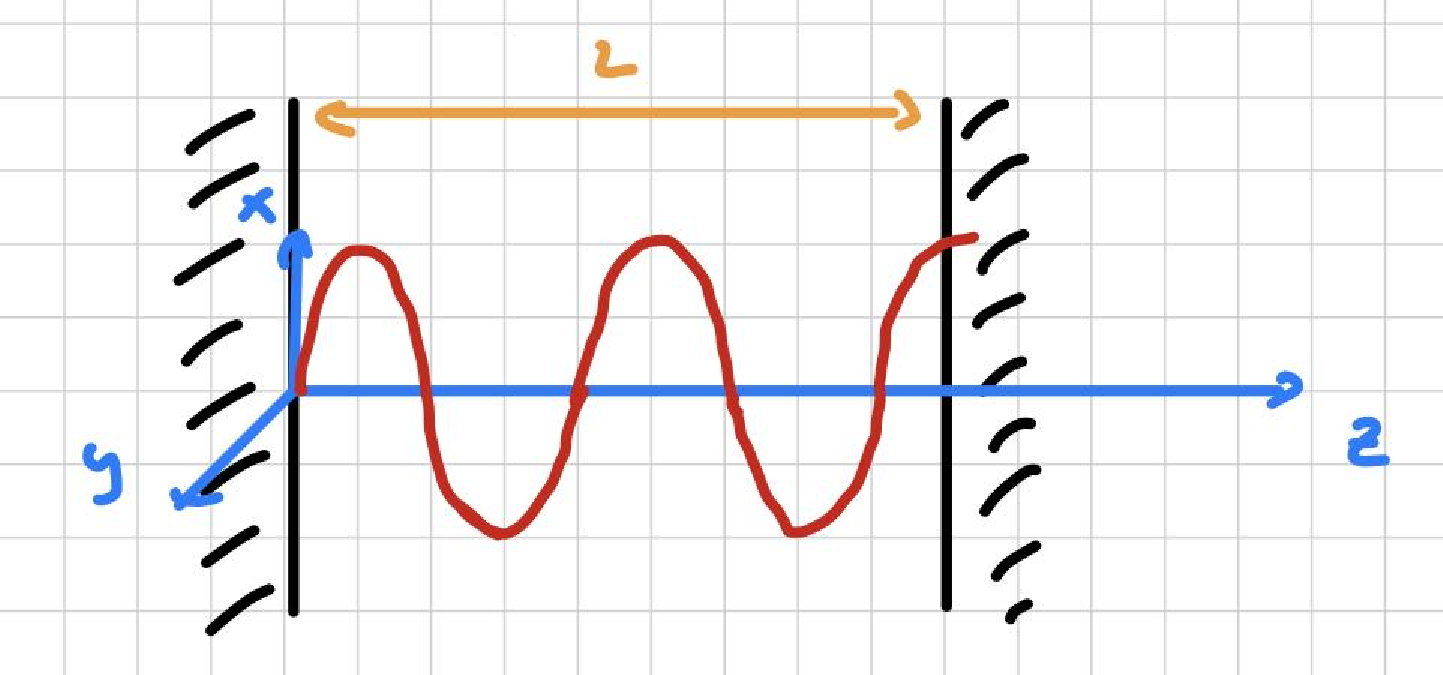
\includegraphics[width=0.6\linewidth]{images_in_pdf/11-/Grafico_65.pdf}
\end{figure}

Suppose that:
\begin{itemize}
    \item the radiation field is confined in a one-dimensional cavity along the $z$-axis, with perfectly conducting walls at $z=0$ and $z=L$ (i.e. no field can escape from the cavity);
    \item the boundary condition $\vec{E}=0$ at the walls implies standing waves;
    \item the electric field is polarized along $\hat{x}$;
    \item there are no charges, no currents, and no dielectric material in the cavity, so the field propagates in vacuum.
\end{itemize}

The Maxwell equations in differential form reduce to
\begin{equation}\label{eqn:11-maxwell-eqs}
\begin{cases}
\vec{\nabla}\times\vec{E}=-\pdv{\vec{B}}{t}\\[1ex]
\vec{\nabla}\,\vec{E}=0\\[1ex]
\vec{\nabla}\times\vec{B}=\mu_0\epsilon_0\pdv{\vec{E}}{t}\\[1ex]
\vec{\nabla}\,\vec{B}=0
\end{cases}
\end{equation}

and the electric field of a single mode $m$ can be written as
\begin{equation}\label{eqn:11-single-mode-electric-field}
\begin{aligned}
&\vec{E}_{m}(z,t) = E_{m}(z,t)\,\hat{x} =
\,E_0\sin(k_m z)\sin(\omega_m t)\,\hat{x},\\[1ex]
\text{where:}\hspace{2ex}
&k_m = \frac{m\pi}{L},
\hspace{2ex}
\omega_m=ck_m=\frac{m\pi c}{L},
\hspace{2ex}
m=1,2,3,\dots
\end{aligned}
\end{equation}

in which the allowed frequencies are fixed by the boundary conditions of the cavity.

Since the magnetic field must be orthogonal both to the electric field and to the propagation direction, it follows that:
\begin{gather}
\vec{B}(\vec{r},t) = B_y(z,t)\,\hat{y}\\[1ex]
\vec{\nabla} \times \vec{B} = 
\mu_0 \epsilon_0\, \pdv{\vec{E}}{t} 
\implies - \pdv{B_y}{t} = 
\mu_0 \epsilon_0\, \pdv{E_x}{t} \\[1ex]
\implies B_y(z,t) = B_0 \cos(kz) \cos(\omega t)
\end{gather} 

with $B_0=E_0/c$, so that the two fields satisfy Maxwell equations and are phase-shifted by $\pi/2$.

\subsubsection{Energy and harmonic oscillator analogy}

If we define $V=LA$ as the effective cavity volume, the classical energy of a single mode is
\begin{equation}\label{eqn:11-single-mode-classical-energy}
H_m = \frac12\int_V dV
\left[
    \epsilon_0 E^2_{m}(\vec r,t)+\frac{1}{\mu_0}B^2_{m}(\vec r,t)
\right] =
\frac12\int_V dV
\left[
    \epsilon_0 E_{m,x}^2(z,t)+\frac{1}{\mu_0}B_{m,y}^2(z,t)
\right].
\end{equation}

Separating the electric and magnetic contributions, we obtain
\begin{equation}\label{eqn:11-single-mode-electric-energy}
\begin{split}
    U_{el.} &= \frac{1}{2}\epsilon_0 A\, \int_0^L dz \, E_0^2\, sin^2(kz)\, \sin^2(\omega t) = \\[1ex]
    &= \frac{1}{4}\epsilon_0 A\, E_0^2\, \sin^2(\omega t) \, \int_0^L dz \, [1-\cos(2kz)] = \\[1ex]
    &=\frac{1}{4}\epsilon_0 A\, E_0^2\, \sin^2(\omega t) \, \bigl(L-\frac{\sin(2kL)}{2k}\bigr)
\end{split}
\end{equation}

The term $\sin(2kL)= 0$  for the boundary conditions, so we obtain:
\begin{equation}\label{eqn:11-single-mode-electric-energy-2}
U_{el.}=\frac{1}{4}\epsilon_0\, V\, E_0^2\, \sin^2(\omega t)
\end{equation}

For the magnetic term we have:
\begin{equation}\label{eqn:11-single-mode-magnetic-energy}
\begin{split}
    U_{M} &= \frac{1}{2\mu_0} A\, \int_0^L dz \, B_0^2\, \cos^2(kz)\, \cos^2(\omega t)= \\[1ex]
    &= \frac{1}{4\mu_0} A\, B_0^2\, \cos^2(\omega t) \, \int_0^L dz \, [1+\cos(2kz)]= \\[1ex]
    &=\frac{1}{4\mu_0} A\, B_0^2\, \cos^2(\omega t) \, \bigl(L+\frac{\sin(2kL)}{2k}\bigr) = \\[1ex]
    &= \frac{1}{4\mu_0}\, V\, B_0^2\, \cos^2(\omega t)
\end{split}
\end{equation}

Therefore,
  \[H = U_{el.}+U_M = \frac{V}{4}\biggr[\epsilon_0 \, E_0^2\, \sin^2(\omega t)+\frac{1}{\mu_0}\, B_0^2\, \cos^2(\omega t)\biggr]\]

\calloutinfo{%
Energy is continuously exchanged between the electric and magnetic parts. This is formally analogous to the exchange between kinetic and potential energy in a harmonic oscillator:
\begin{equation}\label{eqn:11-harmonic-oscillator-energy}
H=\frac{p^2}{2m}+\frac12 m\omega^2 x^2.
\end{equation}
}

\subsection{Quantization in the harmonic oscillator picture}\label{subsec:11-quantization-harmonic-oscillator}

\subsubsection{Hamiltonian and Schrödinger equation}

Promoting $H$ to its quantum version $\hat{H}$, we can write the time-independent Schrödinger equation for the field mode:
\begin{equation}\label{eqn:11-time-independent-schrodinger-equation}
\hat H\psi=E\psi,
\hspace{2ex}
\hat H=\frac{1}{2m}\left[\hat p_x^2+m^2\omega^2\hat X^2\right];
\end{equation}

More explicitly, the equation reads:
\begin{equation}\label{eqn:11-schrodinger-eq-harmonic-potential}
-\frac{\hbar^2}{2m}\frac{d^2\psi}{dx^2}+\frac12 m\omega^2x^2\psi=E\psi.
\end{equation}


If we now introduce the normalized variables
\begin{equation}\label{eqn:11-normalized-variables}
\hat q=\sqrt{m}\,\hat X,
\qquad
\hat p=\frac{1}{\sqrt{m}}\hat p_x,
\end{equation}

then the Hamiltonian becomes
\begin{equation}\label{eqn:11-harmonic-oscillator-hamiltonian-normalized}
\hat H=\frac12\left(\hat p^2+\omega^2\hat q^2\right).
\end{equation}

\calloutinfo{%
This shows that a single electromagnetic mode is formally equivalent to a quantum harmonic oscillator, where the mode amplitudes play the role of canonical coordinate and momentum.
}

If we use the correspondence rule\footnote{The correspondence rule states that the predictions of quantum mechanics must seamlessly reduce to those of classical physics} we can replace classical variables with quantized operators:
\begin{equation}\label{eqn:11-quantized-field-operators}
    \begin{cases}
    \hat{q}(t) = \sqrt{\frac{\epsilon_0V}{2\omega^2}}\, E_0 \, \sin(\omega t)\\[1ex]
    \hat{p}(t) = \sqrt{\frac{V}{2\mu_0}}\, B_0 \, \cos(\omega t) =\sqrt{\frac{\epsilon_0V}{2}}\, E_0 \, \cos(\omega t)
\end{cases}
\end{equation}

Where we use $B_0 = \tfrac{E_0}{c}$ and $c = \tfrac{1}{\sqrt{\epsilon_0\mu_0}}$.
If we extend this argument to all modes we can conclude that by studying the problem of an ideal resonant cavity, we have been led to the conjecture that \hl{the radiation field can be viewed as a collection of quantized simple harmonic oscillator}.

\subsubsection{Annihilation and creation operators}

To construct the Hilbert space of the state vectors related to the radiation field, we need to introduce \emph{annihilation} and \emph{creation} operators $\hat{a}$ and $\hat{a}^\dagger$.
\begin{equation}\label{eqn:11-annihilation-creation-operators-1}
\begin{cases}
    \hat{q} =\sqrt{\frac{\hbar}{2m}}\, (\hat{a}+\hat{a}^\dagger)\\[0.5ex]
    \hat{p} = -i\sqrt{\frac{\hbar \omega }{2}}\, (\hat{a}-\hat{a}^\dagger)
\end{cases}
\end{equation}
inverting:
\begin{equation}\label{eqn:11-annihilation-creation-operators-2}
\begin{cases}
    \hat{a} =\frac{1}{\sqrt{2\hbar \omega}}\, (\omega \hat{q}+i\hat{p})\\[0.5ex]
    \hat{a}^\dagger = \frac{1}{\sqrt{2\hbar \omega}}\, (\omega\hat{q}-i\hat{p})
\end{cases}
\end{equation}
in the means of the original position and momentum operators:
\begin{equation}\label{eqn:11-annihilation-creation-operators-3}
\begin{cases}
    \hat{a} =\frac{1}{\sqrt{2\hbar \omega m}}\, (m\omega \hat{X}+i\hat{p}_x)\\[0.5ex]
    \hat{a}^\dagger = \frac{1}{\sqrt{2\hbar \omega m}}\, (m\omega\hat{X}-i\hat{p}_x)
\end{cases}
\end{equation}

which allows us to rewrite the Hamiltonian as
\begin{equation}\label{eqn:11-hamiltonian-annihilation-creation-operators}
\hat{H} = \hbar \omega \, 
\biggl(\hat{a}^\dagger \hat{a}+\frac{1}{2}\bigr)
\end{equation}

\question{But do these operators commute?}{%
No, they do not. We can verify this by direct calculation:

\begin{proof}
We can verify this by direct calculation:

\begin{align}
\hat{a}^\dagger\hat{a} &= \frac{1}{2m\hbar \omega} \, (m\omega \hat{X}-i\hat{p})\, (m\omega \hat{X}+i\hat{p}) \nonumber \\
&= \frac{1}{2m\hbar \omega} \, [\hat{p}^2+(m\omega \hat{X})^2+im\omega(\hat{X}\hat{p}-\hat{p}\hat{X})] \nonumber \\
&=\frac{1}{\hbar \omega}\, \frac{1}{2m}\,[\hat{p}^2+(m\omega\hat{X})^2]+ \frac{i}{2\hbar}\, [\hat{X},\hat{p}] \nonumber \\
&=\frac{1}{\hbar\omega}\, \hat{H} -\frac{1}{2} \rlap{\hspace{2cm}\text{given } $[\hat{X},\hat{p}]= i\hbar$} \label{eqn:11-commutation-annihilation-creation-operators-proof-1}
\end{align}

Similarly, it can be proven that:
\begin{equation}\label{eqn:11-commutation-annihilation-creation-operators-proof-2}
    \hat{a}\hat{a}^\dagger = 
    \frac{1}{\hbar \omega}\, \hat{H} +\frac{1}{2}
\end{equation}

Therefore:
\begin{equation}\label{eqn:11-commutation-annihilation-creation-operators}
[\hat{a},\hat{a}^\dagger]= \hat{a}\hat{a}^\dagger - \hat{a}^\dagger\hat{a} = 1
\end{equation}
\end{proof}
}

\callout{Proposition: all eigenvalues of $\hat{H}$ are positive}{%
The structure of the Hilbert space is determined by the fact that $\hat{H}$ is a positive operator:
\begin{equation}\label{eqn:11-H-is-positive-operator}
\bra{\psi}\hat{H}\ket{\psi} \geq 0
\end{equation}

For any wawefunction $\psi \in \mathcal{H}$.

\begin{proof}
If we set $\ket{f}=\hat{a}\, \ket{\psi}$ and use $\braket{f|f}\geq 0$:

\begin{equation}\label{eqn:11-H-is-positive-operator-proof}
\begin{split}
    \braket{\psi|\hat{H}|\psi}  &= \hbar \omega \, \braket{\psi|\hat{a}^\dagger\hat{a}|\psi} +\frac{\hbar \omega}{2} = \\
    &=\hbar \omega \braket{f|f} + \frac{\hbar \omega}{2} \geq0\\
\end{split}
\end{equation}
The eigenvalues of $\hat{H}$ are not negative!
\end{proof}
}

\subsubsection{Rising and lowering effects of the annihilation and creation operators}

Given that 
\begin{equation}
    [\hat{H},\hat{a}] = \hat{H}\hat{a}-\hat{a}\hat{H} \implies \hat{H}\hat{a} = [\hat{H},\hat{a}]+\hat{a}\hat{H}
\end{equation}
and if $\ket{u}$ is an eigenstate of $\hat{H}$ with eigenvalue $W$:
\begin{equation}
\hat{H}\hat{a}\, \ket{u} = [\hat{H},\hat{a}]\, \ket{u}+\hat{a}\hat{H}\, \ket{u} = [\hat{H},\hat{a}]\, \ket{u}+\hat{a}W\, \ket{u}
\end{equation}

But: 
\begin{equation}\label{eqn:11-commutator-H-a}
    [\hat{H},\hat{a}] = \hbar \omega [\hat{a}^\dagger\hat{a}, \hat{a}]+
    \bigl[\frac{\hbar \omega }2{,\hat{a}}\bigr]
\end{equation}

The second term is clearly zero, while the first one can be rewritten as:
\begin{equation}
\begin{split}
    [\hat{a}^\dagger\hat{a},\hat{a}] &= \hat{a}^\dagger\hat{a}\hat{a}- \hat{a}\hat{a}^\dagger\hat{a} = \\
    &=\hat{a}^\dagger\hat{a}\hat{a}-\hat{a}^\dagger\hat{a}\hat{a}+\hat{a}^\dagger\hat{a}\hat{a}- \hat{a}\hat{a}^\dagger\hat{a} = \\
    &=\hat{a}^\dagger(\hat{a}\hat{a}-\hat{a}\hat{a})+(\hat{a}^\dagger\hat{a}-\hat{a}\hat{a}^\dagger)\hat{a} = \\
    &=\hat{a}^\dagger[\hat{a},\hat{a}]+[\hat{a}^\dagger,\hat{a}]\hat{a} = \\
    &=\hat{a}^\dagger\, 0 -1\, \hat{a} = \\
    &= - \hat{a}
\end{split}
\end{equation}

so the \eqref{eqn:11-commutator-H-a} becomes:
\begin{equation}
[\hat{H},\hat{a}]= -\hbar \omega \hat{a}
\end{equation}

which means that:
\begin{equation}
\begin{split}
    \hat{H}\hat{a} \, \ket{u} &= 
    -\hbar \omega \hat{a}\, \ket{u}+ \hat{a}\hat{H}\, \ket{u} = \\
    &= -\hbar \omega \hat{a}\, \ket{u}+ E_u\hat{a}\, \ket{u} = \\
    &= (E_u -\hbar \omega) \hat{a}\, \ket{u}\\
\end{split}
\end{equation}

in other words,$\hat{H}\hat{a}\, \ket{u}$ is also eigenstate of $\hat{H}$ with eigenvalue $(E_u-\hbar\omega)$, meaning that the effect of $\hat{a}$ is \textbf{lowering} the energy by a quantity $\hbar \omega$. Repeating this process indefinitely would lead to negative energy, but this is not possible: the hamiltonian $\hat{H}$ must have a lowest energy eigenstate $\ket{0}$ such that:
\begin{equation}\label{eqn:11-ground-state}
\begin{cases}
    \hat{a}\, \ket{0} = 0,\\
    \bra{0}\, \hat{a}^\dagger = 0;
\end{cases}
\end{equation}

which has energy:
\begin{equation}\label{eqn:11-ground-state-energy}
    \hat{H}\, \ket{0} = \hbar \omega \bigl(\hat{a}^\dagger\hat{a}+\frac{1}{2}\bigr) \, \ket{0} = \frac{\hbar \omega}{2}\, \ket{0}
\end{equation}

We can apply the same logic to the adjoint operator $\hat{a}^\dagger$ to obtain:
\[\hat{H}\hat{a}^\dagger\, \ket{u} = (E_u+\hbar\omega)\hat{a}^\dagger\, \ket{u}\]
which means that $\hat{a}^\dagger$ \textbf{raises} the energy by a quantity $\hbar \omega$.

\subsubsection{Number operator and photon number states}

Although the equations describing electromagnetic and mechanical oscillators share the identical mathematical form, for electromagnetic fields the focus shifts from the oscillators themselves to their quanta of excitation. 

\calloutinfo{%
    Following Einstein's hypothesis that the electromagnetic field is composed of \textbf{discrete quanta}, the term \say{quantum of excitation of the E.M. field} can be replaced by \say{photon}, treating them as physical entities on the same footing as massive particles. 
}

In this framework, the ground state of the radiation oscillator is referred to as the \textbf{vacuum state}, which contains no photons.

The product $\hat{a}^\dagger\hat{a}$ is called \textbf{number operator: $\hat{n} =\hat{a}^\dagger\hat{a} $}

\begin{equation}\label{eqn:11-eigenvalue-equation-number-operator-1}
    \hat{H} \, \ket{n} = E_n \, \ket{n} = \hbar \omega 
    \bigl(\hat{a}^\dagger\hat{a}+\frac{1}{2}\bigr)\, \ket{n}
\end{equation}

multiplying both sides by $\hat{a}^\dagger$ we obtain:
\begin{equation}\label{eqn:11-eigenvalue-equation-number-operator-2}
\begin{split}
    \hbar \omega 
    \bigl(
        \hat{a}^\dagger(\hat{a}^\dagger\hat{a})+\frac{1}{2}\hat{a}^\dagger
    \bigr) \, \ket{n} 
    &= E_n \hat{a}^\dagger \, \ket{n} \\[0.5ex]
    \hbar \omega 
    \bigl(
        \hat{a}^\dagger(\hat{a}\hat{a}^\dagger-1)+\frac{1}{2}\hat{a}^\dagger
    \bigr)\, \ket{n} 
    &= E_n \hat{a}^\dagger \, \ket{n} \\[0.5ex]
    \hbar \omega 
    \bigl(
        \hat{a}^\dagger\hat{a}+\frac{1}{2}-1
    \bigr)\hat{a}^\dagger\, \ket{n} 
    &= E_n \hat{a}^\dagger \, \ket{n} \\[0.5ex]
    \hbar \omega 
    \bigl(
        \hat{a}^\dagger\hat{a}+\frac{1}{2}
    \bigr)\hat{a}^\dagger\, \ket{n} 
    &= (E_n+\hbar \omega ) \hat{a}^\dagger \, \ket{n}\\[0.5ex]
    \hat{H}\hat{a}^\dagger\, \ket{n} 
    &= (E_n+\hbar\omega)\, \hat{a}^\dagger \, \ket{n}
\end{split}
\end{equation}

This means that $\hat{a}^\dagger\, \ket{n}$ is an eigenstate of energy with eigenvalue $(E_n + \hbar \omega)$. This is precisely why $\hat{a}^\dagger$ is called \text{creation operator}, since its action is to \textbf{create a photon of energy $\hbar\omega$}.

If we repeat the same procedure, but this time multiplying by $\hat{a}$, we obtain:
\begin{equation}\label{eqn:11-eigenvalue-equation-number-operator-3}
\hat{H}\hat{a}\, \ket{n} = (E_n-\hbar \omega) \hat{a}^\dagger\, \ket{n}
\end{equation}

in a similar fashion, $\hat{a}$ is called \textbf{annihilation operator} because \textbf{it destroys a photon of energy $\hbar\omega$}.

Since $E_{n+1} = E_n+\hbar\omega$:
\begin{equation}\label{eqn:11-energy-eigenvalues-number-states}
E_n = \hbar \omega \bigl(n+\frac{1}{2}\bigr) \hspace{0.5cm} n = 0,1,2,3,...
\end{equation}

Within this picture, the eigenvectors of $\hat{n}=\hat{a}^\dagger\hat{a}$ are called \textbf{number states} $\ket{n}$:
\begin{equation}\label{eqn:11-number-states}
\hat{n} \, \ket{n} = n\, \ket{n} \hspace{1cm} \braket{n|n'} = \delta_{n,n'}
\end{equation}

The action of the annihilation operator on a number state $\ket{n}$ produces a new state proportional to $\ket{n-1}$. We can determine the proportionality constant $C_n$ through the following derivation:
\begin{align}
    \hat{a} \ket{n} &= C_n \ket{n-1} \label{eqn:11-annihilation-operator-number-state} \\[1ex]
    \left(\bra{n}\hat{a}^\dagger\right) \left(\hat{a}\ket{n}\right) &= \left(C_n^* \bra{n-1}\right) \left(C_n \ket{n-1}\right) \nonumber \\
    \braket{n|\hat{a}^\dagger\hat{a}|n} &= |C_n|^2 \braket{n-1|n-1} \nonumber \\
    \braket{n|\hat{n}|n} &= |C_n|^2 \nonumber \\
    n \braket{n|n} &= |C_n|^2 \implies |C_n| = \sqrt{n} \nonumber
\end{align}

Choosing the phase such that $C_n$ is real, we obtain the \hl{standard action of the \textbf{ladder operators}} on the number states:
\begin{equation}\label{eqn:11-ladder-operators-number-states}
\hat{a} \ket{n} = \sqrt{n} \ket{n-1}, \qquad \hat{a}^\dagger \ket{n} = \sqrt{n+1} \ket{n+1}
\end{equation}

Any number state $\ket{n}$ can be built up from the ground state $\ket{0}$ by the repeated application of the creation operator $\hat{a}^\dagger$:
\begin{equation}\label{eqn:11-number-state-recursive-construction}
\ket{n} = \frac{(\hat{a}^\dagger)^n}{\sqrt{n!}} \ket{0}
\end{equation}

The Hilbert space $\mathcal{H}$ for a single cavity mode is spanned by the number states, meaning that any generic state $\ket{\psi} \in \mathcal{H}$ can be expressed as a linear combination of them:
\begin{equation}\label{eqn:11-generic-state-number-states}
\ket{\psi} = \sum_{n=0}^{\infty} C_n \ket{n}
\end{equation}

This space is known as the \textbf{Fock space}. Since the number states form an orthonormal basis\footnote{Number states are eigenstates of the number operator, which is hermitian, hence they form a complete orthonormal basis.}, the expansion coefficients are given by the projections $C_n = \braket{n|\psi}$, allowing us to write:
\begin{equation}\label{eqn:11-generic-state-number-states-2}
\ket{\psi} = \sum_{n=0}^{\infty} \ket{n}\braket{n|\psi}
\end{equation}

Where appears the \textbf{projection operator} $\sum_{n=0}^{\infty} \ket{n}\bra{n} =\mathcal{I}$.

\calloutwarn{%
Observe that a number state $\ket{n}$ is \textbf{not} a state of a well-defined electric field! 
Let's see why by looking at the field operators and their statistical properties:
\begin{align}
    \hat{E}_x(z,t) &= A_0 (\hat{a} + \hat{a}^\dagger) \sin(kz) \nonumber \\
    \hat{B}_y(z,t) &= B_0 \frac{1}{i} (\hat{a} - \hat{a}^\dagger) \cos(kz) \nonumber
\end{align}
where $A_0$ and $B_0$ are normalization constants. 

Here we remembered the analogy between the field operators and the position and momentum operators of a harmonic oscillator, which allows us to express them in terms of the ladder operators $\hat{a}$ and $\hat{a}^\dagger$:
\begin{equation}\label{eqn:11-field-analogy-ladder-operators}
\hat{a}^\dagger\hat{a} \to \vec{E},\vec{B} \to \hat{p},\hat{q}
\end{equation}

If we compute the expectation value of the electric field in a number state $\ket{n}$, we get:
\begin{align}
    \braket{n|\hat{E}_x|n} &= A_0 \sin(kz) \left[ \braket{n|\hat{a}|n} + \braket{n|\hat{a}^\dagger|n} \right] \nonumber \\
    &= A_0 \sin(kz) \left[ \sqrt{n}\braket{n|n-1} + \sqrt{n+1}\braket{n|n+1} \right] = 0 \nonumber
\end{align}
The average field is identically zero! But does this mean the field is not there? No! Let's look at the expectation value of the square of the field, $\braket{n|\hat{E}_x^2|n}$:
\begin{align}
    \braket{n|\hat{E}_x^2|n} &= A_0^2 \sin^2(kz) \braket{n| (\hat{a}+\hat{a}^\dagger)^2 |n} \nonumber \\
    &= A_0^2 \sin^2(kz) \braket{n| \hat{a}^2 + (\hat{a}^\dagger)^2 + \hat{a}\hat{a}^\dagger + \hat{a}^\dagger\hat{a} |n} \nonumber \\
    &= A_0^2 \sin^2(kz) \left[ 0 + 0 + \braket{n| 1 + 2\hat{a}^\dagger\hat{a} |n} \right] \nonumber \\
    &= A_0^2 \sin^2(kz) (2n + 1) = 2 A_0^2 \sin^2(kz) \left(n + \frac{1}{2}\right) \neq 0 \label{eqn:11-field-fluctuations-n}
\end{align}

\textbf{Crucial point:} The expectation value of the field is zero, but its fluctuations are NOT!
\begin{align}
    \braket{\Delta\hat{E}_x^2(z,t)} &= \braket{\hat{E}_x^2} - \braket{\hat{E}_x}^2 = 2 A_0^2 \sin^2(kz) \left(n + \frac{1}{2}\right) \nonumber \\
    \sigma_{E} = \sqrt{\braket{\Delta\hat{E}_x^2}} &= \sqrt{2} A_0 |\sin(kz)| \left(n + \frac{1}{2}\right)^{\frac{1}{2}} \nonumber
\end{align}

Even for $n=0$ (the ground state), the field fluctuations are strictly non-zero! These are the \textbf{vacuum fluctuations}, which deeply show that the quantum vacuum is not an empty, dead space, but it actively contains zero-point energy fluctuations of the electromagnetic field.

This behavior is completely dictated by the \textbf{Uncertainty Principle}. Indeed, the photon number operator and the electric field do not commute:
\[
[\hat{n}, \hat{E}_x] = A_0 \sin(kz) (\hat{a} - \hat{a}^\dagger) \neq 0
\]
Since any two generic operators satisfying $[\hat{A},\hat{B}] = \hat{C}$ must obey the uncertainty relation $\Delta \hat{A} \, \Delta \hat{B} \geq \frac{1}{2}|\braket{\hat{C}}|$, for our physical observables we find:
\[
\Delta \hat{n} \, \Delta \hat{E}_x \geq \frac{1}{2} A_0 |\sin(kz)| \, |\braket{n| \hat{a} - \hat{a}^\dagger |n}|
\]
\textbf{Take-away message:} In a number state, the photon number is perfectly sharp ($\Delta \hat{n} = 0$), which forces the electric field amplitude to become completely uncertain ($\Delta \hat{E}_x \to \infty$). If you want a well-defined field amplitude (like in a classical laser beam), you must accept uncertainty in the photon number. This is exactly why classical-like light cannot be described by number states, but requires \textbf{coherent states}.
}

\subsection{Quadrature operators}
Given the single-mode electric field operator:
\begin{equation}\label{eqn:11-single-mode-field-time}
\hat{E}_x(z,t) = A_0\left(\hat{a}e^{-i\omega t}+\hat{a}^\dagger e^{i\omega t}\right) \sin(kz),
\end{equation}

we can introduce the dimensionless \textbf{quadrature operators} defined at $t=0$:
\begin{equation}\label{eqn:11-quadrature-operators}
\begin{cases}
\hat{x}_1 = \dfrac{1}{2}\left(\hat{a}+\hat{a}^\dagger\right),\\[1.5ex]
\hat{x}_2 = \dfrac{1}{2i}\left(\hat{a}-\hat{a}^\dagger\right),
\end{cases}
\qquad \implies \qquad [\hat{x}_1,\hat{x}_2]=\dfrac{i}{2}.
\end{equation}

By expanding the exponentials via Euler's formula, the time-dependent electric field can be elegantly expressed as:
\begin{equation}\label{eqn:11-electric-field-quadrature-operators}
\hat{E}_x(z,t) = 2A_0\sin(kz) \bigl[ \hat{x}_1\cos(\omega t) + \hat{x}_2\sin(\omega t) \bigr].
\end{equation}

The operators $\hat{x}_1$ and $\hat{x}_2$ correspond to the two field quadratures, representing the two independent out-of-phase amplitudes of the electromagnetic mode. They are directly related to the standard canonical position and momentum operators $(\hat{q}, \hat{p})$ of the mechanical analogue oscillator:
\begin{equation}\label{eqn:11-quadrature-operators-canonical-variables}
\begin{cases}
\hat{x}_1 = \sqrt{\dfrac{m\omega}{2\hbar}}\,\hat{q},\\[1.5ex]
\hat{x}_2 = \sqrt{\dfrac{1}{2m\hbar\omega}}\,\hat{p}.
\end{cases}
\end{equation}

We can now evaluate the product of their quantum uncertainties. By explicit substitution of the scaling factors, the mass $m$ and frequency $\omega$ cancel out perfectly:
\begin{align}
    \Delta \hat{x}_1 \, \Delta \hat{x}_2 &= \sqrt{\frac{m\omega }{2\hbar}}\, \Delta\hat{q} \cdot \sqrt{\frac{1}{2m\hbar \omega}}\, \Delta \hat{p} \nonumber \\
    &= \frac{1}{2\hbar}\, \Delta\hat{q} \, \Delta\hat{p}. \label{eqn:11-quadrature-uncertainty-derivation}
\end{align}

By invoking the fundamental Heisenberg uncertainty relation for canonical coordinates, $\Delta\hat{q} \, \Delta\hat{p} \geq \frac{\hbar}{2}$, we immediately find the lower bound for the quadrature fluctuations:
\begin{equation}\label{eqn:11-quadrature-uncertainty-final}
    \Delta \hat{x}_1 \, \Delta \hat{x}_2 \geq \frac{1}{2\hbar} \left( \frac{\hbar}{2} \right) \implies \Delta \hat{x}_1 \, \Delta \hat{x}_2 \geq \frac{1}{4}.
\end{equation}
\hspace{1ex}
\calloutinfo{%
This is the physical insight of Equation~\eqref{eqn:11-quadrature-uncertainty-final} to be remembered: the field quadratures are strictly subject to a minimum-uncertainty relation. This implies that the \textbf{amplitude and the phase} (and consequently, the field direction in the complex amplitude plane) \textbf{cannot be simultaneously known} with arbitrary precision. Any attempt to squeeze the noise in one quadrature will inevitably amplify the fluctuations in the orthogonal one.
}

\begin{figure}[H]
    \centering
    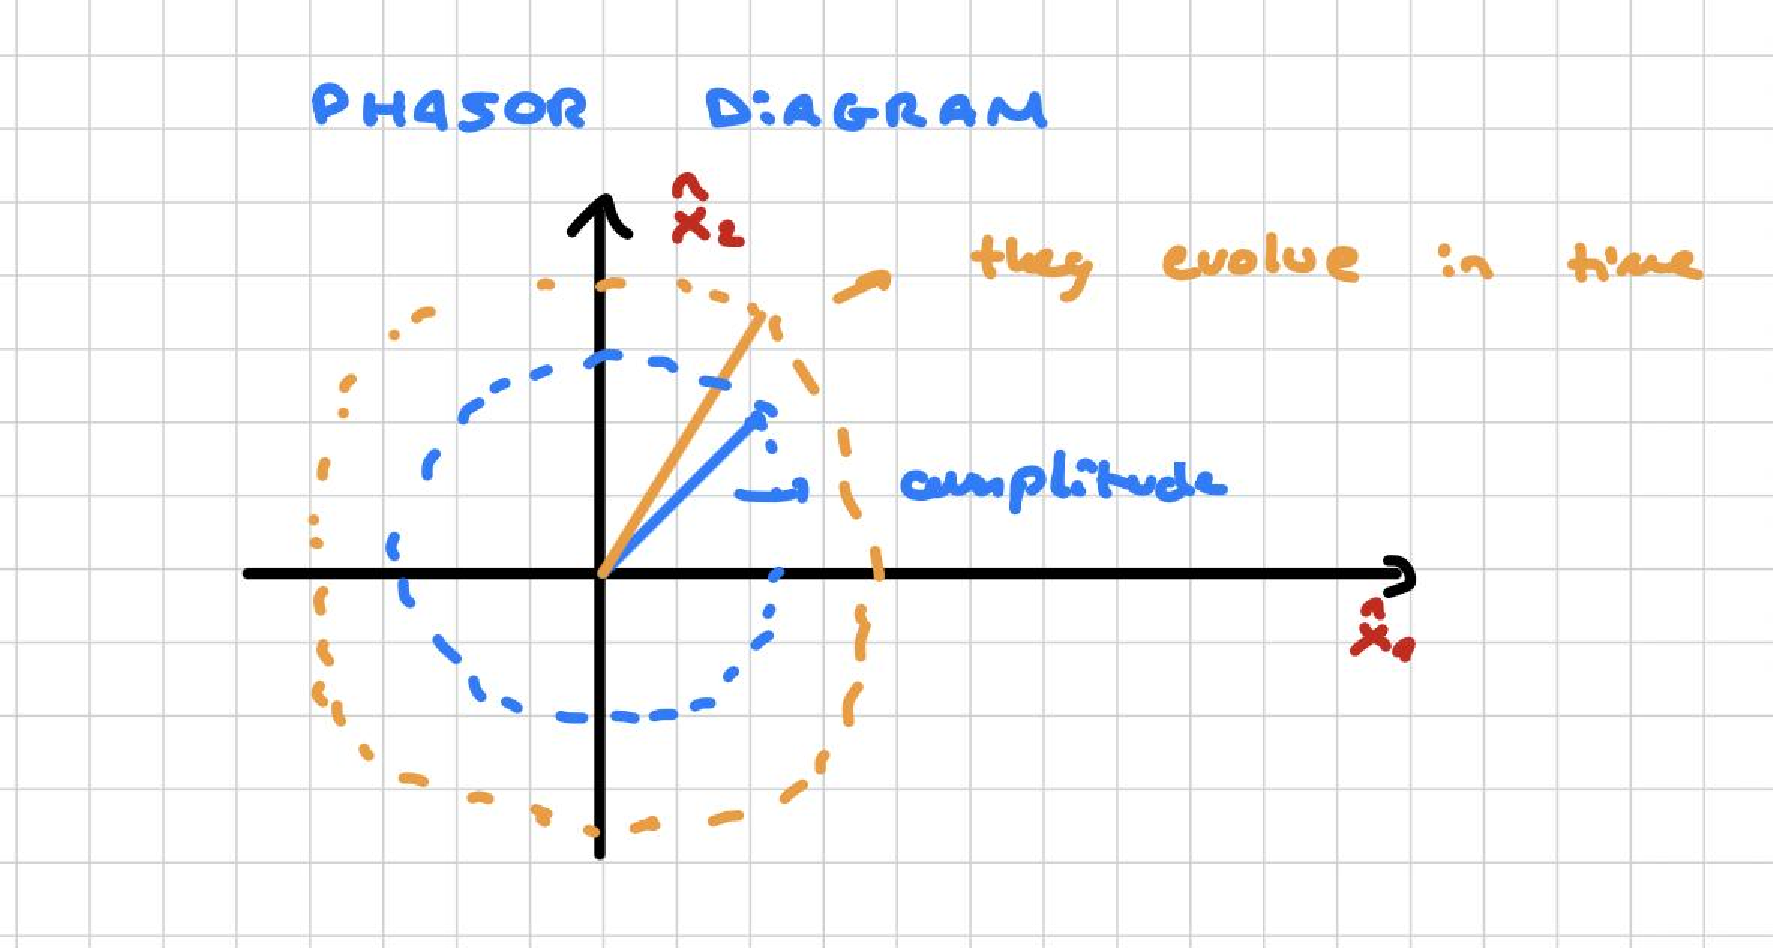
\includegraphics[width=0.6\linewidth]{images_in_pdf/11-/Grafico_66.pdf}
\end{figure}

For the \textbf{number state:}
\begin{equation}\label{eqn:11-number-state-quadratures}
\begin{split}
    \braket{n|\hat{x}_1|n} &= \braket{n|\hat{x}_2|n} =0\\\\
    \braket{n|\hat{x}_1^2|n} &= \frac{1}{4}\, \braket{n| (\hat{a}^\dagger)^2 + \hat{a}^2 + \hat{a}^\dagger\hat{a}+\hat{a}\hat{a}^\dagger|n}\\
    &=\frac{1}{4}\, (0+0+\braket{n|1+2\hat{a}^\dagger\hat{a}|n})\\
    & = \frac{1}{4}\, (1+2n) = \braket{n|\hat{x}_2^2|n} 
\end{split}
\end{equation}

This again shows that the average value of each quadrature vanishes, but the fluctuations do not. In particular, for the vacuum state, \hl{the uncertainties in quadratures operators are the same and the vacuum state, having $n=0$, minimizes the uncertainty product:}
\begin{equation}\label{eqn:11-vacuum-state-quadrature-uncertainties}
\braket{(\Delta \hat{x}_1)^2}_\text{vacuum} =\braket{(\Delta \hat{x}_2)^2}_\text{vacuum} = \frac{1}{4} 
\end{equation}

\begin{figure}[H]
    \centering
    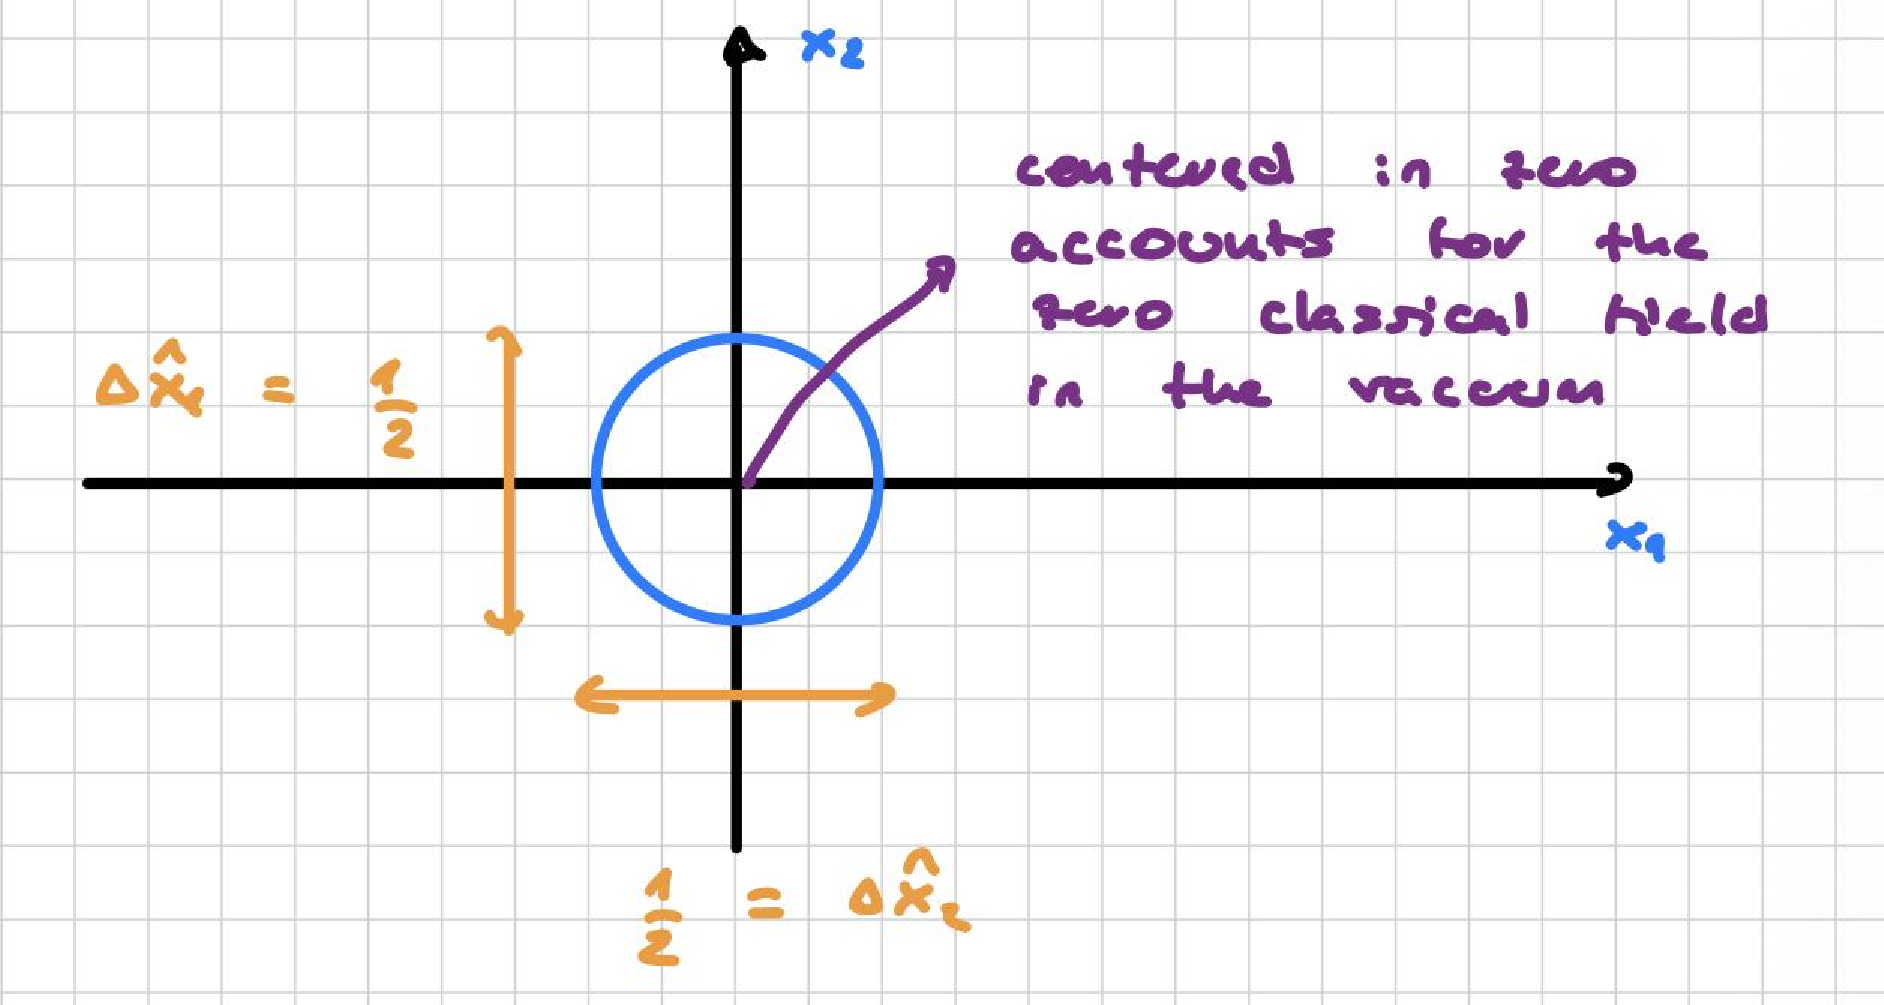
\includegraphics[width=0.6\linewidth]{images_in_pdf/11-/Grafico_67.pdf}
\end{figure}

\calloutinfo{%
States that satisfy
\begin{equation}\label{eqn:11-minimum-uncertainty-states}
\Delta \hat{x}_1\,\Delta \hat{x}_2=\frac{1}{4}
\end{equation}

are called \textbf{minimum-uncertainty states} (Eqn~\eqref{eqn:11-minimum-uncertainty-states}). The vacuum is one example, but \textbf{coherent states} also belong to this class.
}